\documentclass[a4paper, 10pt, final, garamond]{book}
\usepackage{cours-preambule}

\makeatletter
\renewcommand{\@chapapp}{Devoir surveill\'e -- num\'ero}
\makeatother

\begin{document}
\setcounter{chapter}{2}

\chapter{Commentaires sur le DS n\degree03}

\section{Commentaires généraux}
Un DS réussi de manière globalement homogène et bien réussi par ailleurs.
Quelques notions sont encore peu acquises (distinction $p\ind{tot}$ et $p_0$ ou
$p^\circ$~; volume en \si{m^3} et pas en \si{L} pour les gaz parfaits~; dérivée
d'une fonction et non pas d'un nombre~; traitement des ressorts…), mais sinon
l'ensemble est solide. Peu d'étudiant-es tentent leur chance sur les questions
plus compliquées, mais les questions typique de cours (RLC~: équation
différentielle et résolution) sont maîtrisées. Très peu de malus, bravo~! Il n'y
a pas vraiment de fossé au sein-même de la classe comme c'était le cas au DS02,
et le niveau général s'est amélioré. Continuez ainsi~!

\begin{center}
	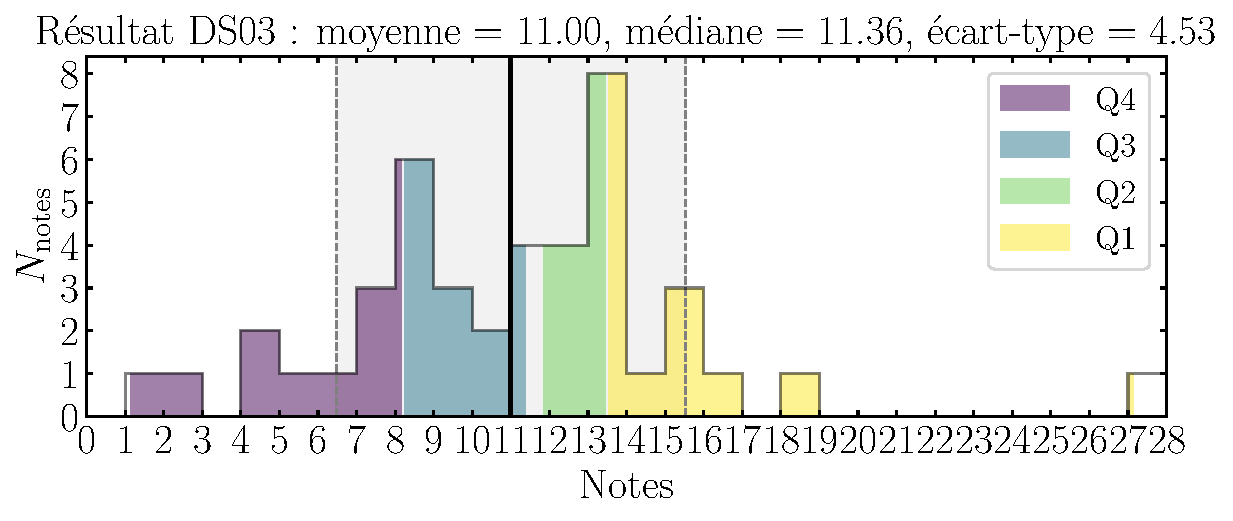
\includegraphics[width=\linewidth]{DS03_rslt.pdf}
\end{center}

\setcounter{section}{0}
\exercice[23]{Pentachlorure de phosphore}
\begin{enumerate}
	\nitem{3}%
	Attention à la conversion. TB sinon.
	\nitem{5}%
	TB dans l'ensemble. Presqu'aucune colonne $n\ind{tot, gaz}$
	d'oubliée.
	\nitem{3}%
	Victime de vos connaissances~: loi de \textsc{Dalton} bien citée
	mais inutile ici. Faites la distinction entre toutes les grandeurs~:
	$P\ind{tot, gaz} \neq p_0 \neq p^\circ$~!
	\nitem{9}%
	Question tiroir selon votre réponse à Q3…
	\nitem{3}%
	Bien globalement.
\end{enumerate}

\exercice[42]{États finaux variés}
\begin{enumerate}
	\nitem{3}%
	On pouvait galérer à écrire les réactions, mais utiliser les
	relations entre réactions et constantes était plus simple et plus rapide.
	\nitem{10}%
	Bien dans l'ensemble. Attention aux signes (faux dans le corrigé
	par ailleurs, cf.\ nouvelle version en ligne). Déterminer l'état $\Lra$ donner
	les concentrations de chaque constituant~!
	\nitem{6}%
	Soit manque de tableau pour faire du clair dans les idées, soit un
	oubli flagrant de la puissance 2 sur le coefficient stœchiométrique pour
	\ce{HO-}.
	\nitem{3}%
	Bien.
	\nitem{4}%
	Ici, ç'aurait été trop long d'écrire toutes les constantes. Il était
	nécessaire de passer par le lien entre réactions et constantes. Il fallait
	réutiliser la réaction (4).
	\nitem{5}%
	Bien (ouf~!).
	\nitem{4}%
	Encore quelques confusions $\xi_{\max}$, $\xi_f$ et $\xi\ind{eq}$,
	mais elles sont rares.
	\nitem{4}%
	Idem. Plus clivante mais mieux réussi que la 7.
	\nitem{3}%
	3 bonnes réponses sur 4 tentatives. Pas mal comme ratio, mais
	dommage pour le manque de tentatives.
\end{enumerate}

\setcounter{section}{0}
\prblm[60]{Amortissement et facteur de qualité RLC}
\begin{enumerate}
	\nitem{8}%
	Très bien~!
	\nitem{5}%
	Il faut \textbf{montrer} la limite $Q \lessgtr 1/2$.
	\nitem{4}%
	Il fallait voir la partie réelle de la racine comme l'inverse d'un
	temps~; c'est la même chose que pour les solutions d'ordre 1.
	\nitem{9}%
	\textbf{Ce n'est pas parce que $u(0)$ est un nombre que $u'(0) =
			0$~!!} C'est une {\Huge insulte aux mathématiques} que d'énoncer ceci
	comme étant vrai. On l'a déjà explicité, $u$ est une fonction~; $u(0)$
	est la fonction évaluée en ce point, c'est évidemment un nombre. Mais
		{\Large
			\[
				\boxed{u'(0) \neq (u(0))'}
			\]
		}
	\nitem{5}%
	Oula. Il faut y aller à tête reposée. Essayez plus.
	\nitem{7}%
	De bonnes idées, mais grosses erreurs d'homogénéité. Il faut
	comparer des choses comparables~: $L/R_0 \ll 1$ ne veut \textbf{rien} dire.
	\nitem{4}%
	Dommage.
	\nitem{2}%
	C'était quand même facile.
	\nitem{3}%
	Bien pour le lien entre oscillations et facteur de qualité, mais ça
	c'est pour le temps de réponse à 95\%~: ici ça serait à \SI{0.20}{V}, ce qui
	fait bien 6 oscillations. Personne n'a utilisé le décrément et la lecture des
	maxima.
	\nitem{4}%
	Quelques recherches prometteuses, mais la réflexion n'a pas décollé.
	\nitem{9}%
	Aucune réponse ici.
\end{enumerate}

\prblm[58]{Assemblages de ressorts}
\begin{enumerate}
	\nitem{4}%
	Attention aux définitions~: $\Ff\ind{rap} = \pm k
		(\boxed{\ell-\ell_0})\uz$, c'est bien $\ell_0$ et pas $\ell\ind{eq}$~!
	Ça n'a pas de sens d'introduire une notation $x = \ell - \ell_0$ quand on
	étudie un système sur l'axe $z$ uniquement…
	Pourquoi des frottements~? Vous aimez souffrir~? Bon, vous êtes en prépa, donc
	évidemment oui, mais si c'est pas dit ne vous en rajoutez pas.
	\nitem{3}%
	Pas besoin du PFD, on utilise la définition du repos directement.
	\nitem{6}%
	Problème de logique sur cette question. Les forces qui s'appliquent
	à un système sont celles qui agissent directement \textbf{sur} le système. Le
	poids du la masse M ne peut apparaître dans le bilan des forces sur la masse
	N~! La masse N subit \textbf{deux forces de rappel}, comme dans le DM.
	\smallbreak
	Ceci étant dit, à l'équilibre la force de rappel du ressort 2 est égale au
	poids de la masse M~; ainsi mathématiquement la masse N subit le poids de la
	masse M, mais c'est une situation particulière à l'équilibre.
	\nitem{4}%
	Pas de points donnés si détermination de la relation avec mauvais
	bilan des forces.
	\nitem{2}%
	Commenter n'est pas décrire.
	\nitem{4}%
	Déterminer \textbf{puis} simplifier.
	\nitem{3}%
	Attention à l'homogénéité.
	\nitem{2}%
	RAS.
	\nitem{7}%
	Pas trop mal.
	\nitem{10}%
	C'est pas encore ça.
	\nitem{2}%
	RAS.
	\nitem{2}%
	RAS
	\nitem{9}%
	RAS. 4 personnes ont tenté de répondre, une seule avec l'exacte
	bonne idée.
\end{enumerate}

\end{document}
